\chapter{Dataset construction}
\label{cha:dataset}

The research questions formulated in Chapter~\ref{cha:intro} define the requirements for the evaluation dataset. Testing whether multimodal foundation models improve cross-plant generalization requires power histories and numerical weather covariates synchronized with satellite observations available before each forecast origin. The test also requires strict preservation of plant identities, quality labels, and data provenance to prevent information leakage across splits. This chapter describes how records from the United Kingdom and the United States were assembled into a shared sample contract, which places disparate numerical and visual sources onto a common physical timeline. Chapter~\ref{cha:protocol} details the plant partitions and scoring rules that evaluate these samples.

\section{Challenges in building a transfer dataset}

The evaluation in Chapter~\ref{cha:protocol} holds out entire plants. Each record must therefore remain traceable to its source and site after the numerical streams are standardized. Otherwise, windows from the same plant could enter both training and test partitions, making a transfer result impossible to interpret.

The power record also has to distinguish faulty measurements from genuine low generation. An outage, a stuck inverter, and cloud cover can produce similar readings, but they describe different conditions. Quality flags and missing-value masks preserve that distinction; extended gaps remain unavailable instead of becoming interpolated targets that no instrument measured.

Finally, the image paired with a forecast must depict the right location at the right time. A frame captured after the forecast origin would reveal future conditions, while a crop from another site would describe a different scene. The corpus therefore retains site coordinates and frame timestamps, selects images available before the origin, and marks absent frames explicitly. These requirements guide the source selection and construction steps that follow.

\section{Published photovoltaic datasets}

This thesis uses measured plant power as the forecasting target. An irradiance measurement describes incoming sunlight, whereas a power measurement records the output of a particular installation. A forecasting model must learn from that installation's observed response, including differences between plants that remain after capacity normalization. The survey therefore focuses on datasets with plant-level production records and identifies which also provide imagery.

\subsection{Production records without imagery}
These collections provide measured generation and numerical context, but no paired image stream. The UK PV and PVDAQ releases supply the power records used in this thesis; the others show the range of available numerical sources.

Open Climate Fix's UK PV dataset~\cite{ukpv} provides half-hourly metered generation for more than 30,000 systems across Great Britain from 2010 to 2025; a smaller subset also has five-minute readings. It includes approximate site locations, capacities, panel orientation and tilt, and flagged bad-data periods, but no imagery.

The NREL PVDAQ archive~\cite{pvdaq} publishes systems across the United States at sub-hourly resolution, from residential rooftops to utility installations, each with system metadata.

HKUST Rooftop PV~\cite{hkpvdata} covers 60 rooftop systems in Hong Kong at five-minute inverter resolution, with on-site weather and equipment metadata. It is the densest of these collections in both time and instrumentation.

PVOD~\cite{pvod} covers ten plants in China at fifteen-minute resolution. It pairs measured power with local weather observations and numerical weather predictions, and it records orientation and location for each plant.

The Ausgrid solar home collection~\cite{ausgrid} records rooftop generation and household consumption for 300 homes in Sydney at half-hourly resolution over three years, but it lacks weather and plant metadata.

\subsection{Production records paired with images}

These datasets link measured plant output to visual observations of the sky or surrounding cloud field. Their image sources and site coverage determine which forecasting and cross-plant transfer tests they can support.

SKIPP'D~\cite{skippd} pairs one California system with ground-based sky images at one-minute resolution. The imagery is the closest available view of the sky above an array, which suits nowcasting; a single site cannot express a transfer task.

MMSP, released with FusionSF~\cite{fusionsf}, is the closest published comparison to this work. It combines capacity-normalized power from 88 plants in China with Himawari satellite imagery and numerical weather data at hourly resolution. It evaluates forecasting on plants held out from training.

\subsection{Positioning among existing datasets}
\label{sec:dataset-positioning}

Table~\ref{tab:dataset-comparison} places these collections beside the corpus built here.

\begin{table}[htbp]
\centering
\begin{tabular}{@{}llllll@{}}
\hline
Dataset & Region & Sites & Cadence & Span & Inputs \\
\hline
UK PV~\cite{ukpv} & GB & 30,000+ & 5/30 min & 2010--2025 & P, M \\
HKUST PV~\cite{hkpvdata} & Hong Kong & 60 & 5 min & 2 years & P, W, M \\
PVOD~\cite{pvod} & China & 10 & 15 min & 1 year & P, W, M \\
Ausgrid~\cite{ausgrid} & Sydney & 300 & 30 min & 3 years & P, L \\
PVDAQ~\cite{pvdaq} & US & 1865 & Variable & Variable & P, M \\
SKIPP'D~\cite{skippd} & California & 1 & 1 min & 2 years & P, C, G \\
MMSP~\cite{fusionsf} & China & 88 & 1 h & 1.5 years & P, W, S \\
This corpus & UK, US & 110 & 15/30 min & 2019--2020 & P, W, M, S \\
\hline
\end{tabular}
\caption{Published photovoltaic datasets. GB denotes Great Britain. Inputs: P, power; W, weather; M, metadata; L, household load; C, capacity; G, ground sky images; S, satellite images. UK PV has a five-minute subset within its thirty-minute collection. This corpus spans 2019--2020 in the UK and January--September 2019 in the US, with sample-level provenance. MMSP is the closest comparison through its multi-plant power, weather, satellite imagery, and plant-held-out evaluation.}
\label{tab:dataset-comparison}
\end{table}

\section{The corpus built here}

Among the collections surveyed here, none provides the combination of cross-plant evaluation, native-cadence power and imagery, and sample-level provenance used in this thesis. The corpus joins two source tracks under one data contract to supply that setting.

The dataset has two parts. A flat Parquet table holds 1,337,654 numerical records across 35 columns. A packed HDF5 archive holds 4,103,892 image frames in 110 site groups. Keeping them apart leaves the numerical data easy to process while preserving timestamp-exact access to large visual payloads. The first track, in the United Kingdom, contains 100 residential photovoltaic systems from 1 January 2019 through 31 December 2020~\cite{ukpv}. Power is sampled every 30 minutes. The systems have capacities from 1.5 to 4.0 kW and are distributed across the United Kingdom. Satellite frames are available from EUMETSAT sources~\cite{eumetsat}.

The second track combines ten United States NREL PVDAQ systems~\cite{pvdaq} with GOES imagery. It covers January through September 2019 at fifteen-minute cadence, with capacities from 1.8 to 408 kW. That spread brings a different scale of deployment, a different sensor product, and a different geographic context. The results chapter reports an inference-only transfer evaluation on one held-out US plant after resampling power to the same 30-minute cadence used in the UK benchmark. The primary multi-plant benchmark remains the UK evaluation. Table~\ref{tab:data-tracks} summarizes both.

\begin{table}[htbp]
\centering
\begin{tabular}{@{}lccccc@{}}
\hline
Track & Sites & Rows & Power & Images & Capacity \\
\hline
UK & 100 & 1,232,862 & 30 min & 15 min & 1.5 to 4.0 kW \\
US & 10 & 104,792 & 15 min & 15 min & 1.8 to 408 kW \\
\hline
\end{tabular}
\caption{The two data tracks. Power and Images report sampling intervals.}
\label{tab:data-tracks}
\end{table}

Compared with MMSP, the corpus covers two geographic tracks and preserves each source's native cadence: the interval at which its observations were collected. UK power remains half-hourly, US power remains fifteen-minute, and satellite frames retain their own timestamps. A common sample definition specifies which plant, history interval, and future interval belong to a forecast; it does not force all sources onto one sampling frequency. This distinction lets a fourteen-day history or six-hour horizon have the same physical meaning in both tracks. Interpolated values are not treated as new measurements.

Each selected image is linked to its capture time and plant location, allowing its observation time to be verified against the numerical history and forecast origin. The US track spans a wider capacity range than the UK track, alongside different satellite sensor characteristics (GOES-16 versus SEVIRI). Eight held-out US plants provide a cross-region and cross-satellite evaluation, testing whether models trained on UK data generalize when deployed under unfamiliar solar regimes and atmospheric dynamics.

The corpus defines each forecast example as one aligned record. At a forecast origin, it combines recent generation, atmospheric and astronomical covariates, and a visual record of the nearby cloud field. Source identity, UTC timestamps, site coordinates, quality flags, and the local frame index link these inputs to the same plant and forecast window. These fields make their alignment auditable.

Figures~\ref{fig:week-uk} and~\ref{fig:week-us} show representative weeks on their native grids. The common corpus lets windows be defined in physical time and resolved at native cadence while preserving differences between the underlying processes.

\begin{figure}[H]
\centering
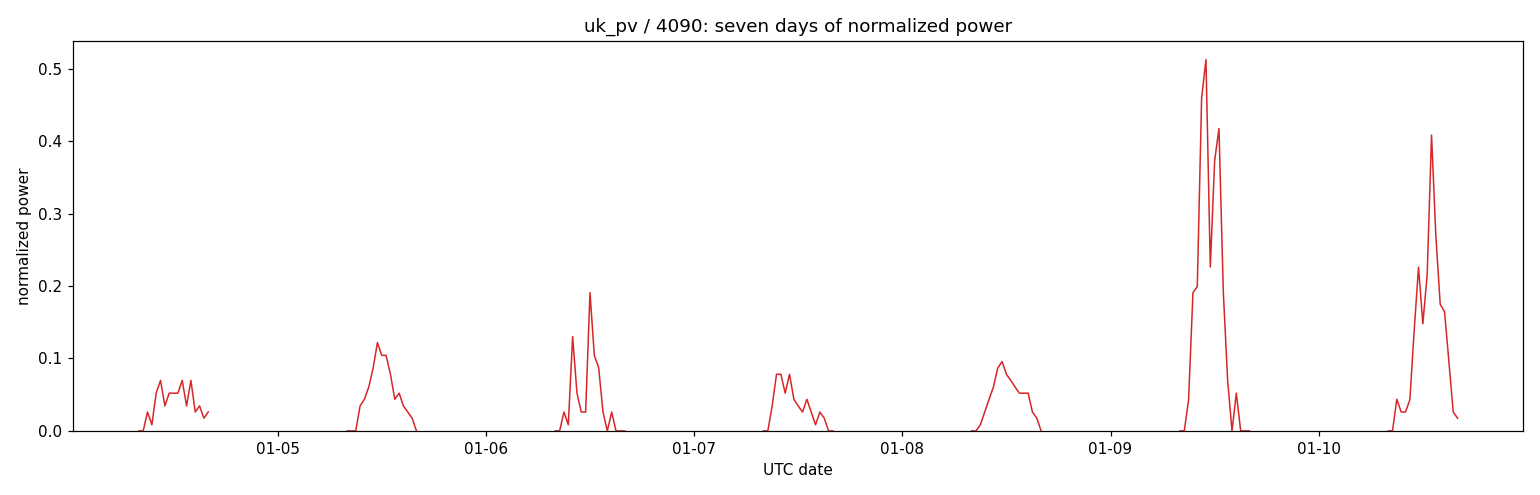
\includegraphics[width=0.92\textwidth]{figures/week_uk_pv.png}
\caption{A representative week from the UK track. The daily envelope is clear, while departures from it vary sharply from one day to the next.}
\label{fig:week-uk}
\end{figure}

\begin{figure}[H]
\centering
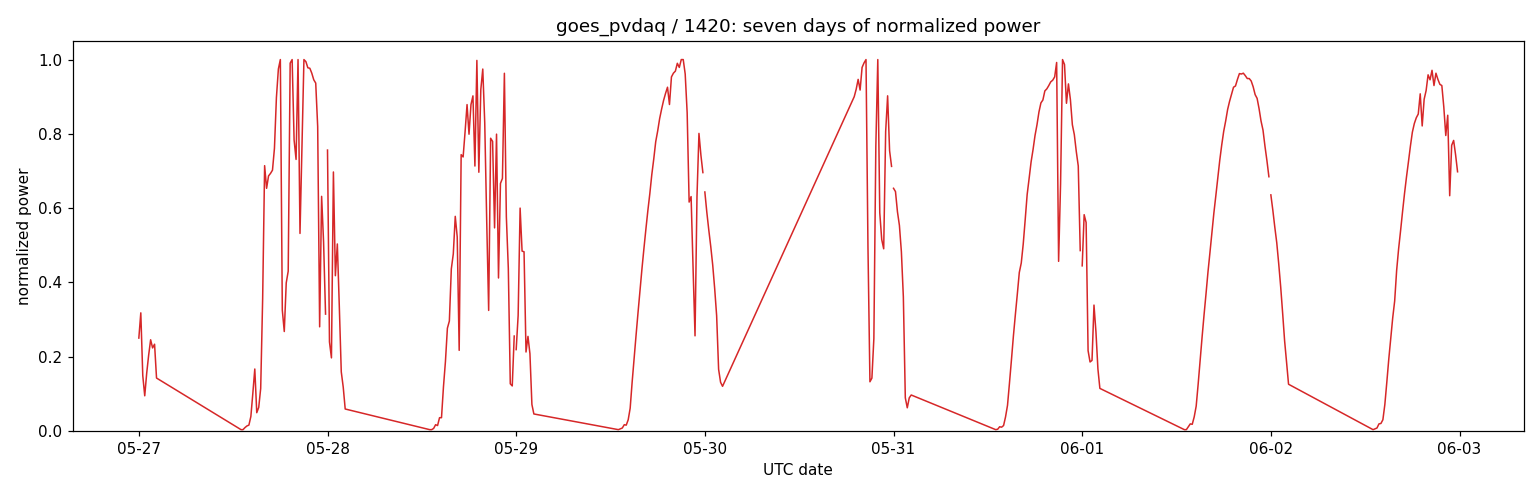
\includegraphics[width=0.92\textwidth]{figures/week_goes_pvdaq.png}
\caption{A representative week from the United States track. The different cadence, capacity range, and data span make this a complementary transfer setting.}
\label{fig:week-us}
\end{figure}

\section{Dataset provenance and harmonization}
\label{sec:provenance}

A corpus assembled from several archives is only credible if every field can be traced to its origin and if the transformations applied along the way are stated. This section names the public sources, then describes the harmonization steps that determine whether records from different countries and instruments can be compared. These steps convert heterogeneous power readings to a common capacity-normalized scale and place every power value, covariate, and satellite frame on one physical timeline.

\subsection{Public sources}

The corpus draws on four public source families. The UK track combines domestic generation measurements~\cite{ukpv} with EUMETSAT satellite imagery~\cite{eumetsat}. The US track pairs NREL PVDAQ records~\cite{pvdaq} with GOES image crops. The Open-Meteo archive provides atmospheric covariates~\cite{openmeteo}. Table~\ref{tab:public-sources} identifies the role of each source.

\begin{table}[htbp]
\centering
\begin{tabularx}{\textwidth}{@{}llY@{}}
\hline
Track & Source & Records \\
\hline
UK power & UK PV & Residential power (30 min), metadata \\
UK imagery & EUMETSAT & Site-centered satellite crops \\
US power & NREL PVDAQ & Power (15 min), metadata \\
US imagery & GOES & Site-centered RGB crops \\
Weather & Open-Meteo & Temperature, radiation, clouds, wind, precipitation \\
\hline
\end{tabularx}
\caption{Public sources combined in the experiment dataset.}
\label{tab:public-sources}
\end{table}

The sources do not arrive on a common clock, grid, or storage format. Each source is checked, cleaned, and standardized before its records are stored in the common dataset format. Dataset construction preserves what was actually observed: power remains at native cadence, images remain in a separate packed archive, and the numerical record stores the metadata needed to select an aligned visual clip.

\subsection{Power and capacity harmonization}

The UK source reports energy over its sampling interval. For the forecasting record, this is converted to power in watts using the interval duration. The United States data already provide a compatible power measure. Both tracks retain measured power and a capacity-normalized target, computed by dividing measured power by the audited installed capacity.

Installed capacity is audited per site and stored with the numerical record. Capacity normalization scales power outputs to the unit interval while preserving local efficiency variations, clipping behavior, and plant-specific shading patterns.

Extended missing intervals remain recorded as unobserved timesteps through quality masks. Avoiding synthetic interpolations prevents imputation artifacts from biasing model training or evaluation.

\subsection{Time, location, and image alignment}

Every numerical row is timestamped in UTC and identifies the plant through its coordinates and source identifiers. The row also contains a direct reference to that plant's imagery. The referenced image archive stores each site's frame sequence with its original timestamps. For a forecast window, selection begins at the numerical forecast origin and retrieves visual slots that precede it.

In the UK track, images arrive at fifteen-minute intervals while power is recorded half-hourly. The loader retrieves the closest valid satellite frame preceding the forecast origin within a 15-minute window, storing the exact image timestamp in the sample record to verify temporal alignment.

\section{Numerical observations}

Each numerical record identifies the dataset, site, UTC timestamp and geographical location. It stores measured power in watts and capacity-normalized power, obtained by dividing the measurement by the audited installed capacity. Outage and stuck-signal observations keep their quality labels, while their normalized targets remain missing rather than being fabricated.

The atmospheric covariates are temperature, shortwave radiation, direct and diffuse radiation, direct normal irradiance, cloud cover, wind speed, and precipitation. Solar and calendar fields include zenith, azimuth, a clear-sky estimate, seasonal sine and cosine terms, and solar time. Table~\ref{tab:numerical-record} lists the full record; Chapter~\ref{cha:protocol} specifies which of these fields each method may use at a forecast origin.

\begin{table}[htbp]
\centering
\begin{tabularx}{\textwidth}{@{}lY@{}}
\hline
Component & Fields \\
\hline
Identity & Dataset, site, UTC time, location, station/camera IDs \\
Target & Measured and capacity-normalized power \\
Weather & Temperature, radiation, cloud cover, wind, precipitation \\
Solar/calendar & Geometry, clear-sky estimate, season, solar time \\
Quality & Outage, stuck-value, night, capacity, site flags \\
Image reference & Timestamp-exact archive index \\
\hline
\end{tabularx}
\caption{Logical structure of a numerical record.}
\label{tab:numerical-record}
\end{table}

\section{Dataset contract}
\label{sec:contract}

The dataset contract defines the contents of one forecasting sample. It preserves the native power and image grids, resolves windows in physical time, and carries the timestamps and validity masks needed to reconstruct each sample. Chapter~\ref{cha:protocol} specifies how those samples are partitioned and scored.

Each logical sample contains normalized power history, a future target, numerical covariates, visual frames, timestamps, plant identity, and masks. The contract defines these fields independently of the model that consumes them; the input choices for each model family are stated in Table~\ref{tab:input-parity}.

The contract also separates values from their validity. A missing power reading, a missing visual slot, and a future target that should not be scored are represented by different masks. Table~\ref{tab:sample-contract} summarizes the fields and their temporal extent. In the model window, a measured zero at night is a valid observation; an absent nighttime row or a faulty reading is not. The loader must preserve that distinction when it constructs the physical-time grid, since replacing missing values with zero would confound absence with observed production.

\begin{table}[htbp]
\centering
\begin{tabularx}{\textwidth}{@{}llY@{}}
\hline
Element & Extent & Role \\
\hline
Power history & 14 days & Local plant context \\
Target & 6 hours & Future power \\
Covariates & History + horizon & Archived weather, solar and calendar fields \\
Visual clip & Recent window & Cloud structure \\
Masks/times & Whole sample & Validity, alignment, provenance \\
\hline
\end{tabularx}
\caption{Logical elements of a forecasting sample.}
\label{tab:sample-contract}
\end{table}

Since the dataset has two power cadences, a fixed number of observations does not mean the same physical history in each track. Defining the task in physical time avoids an accidental advantage for a model evaluated at a coarser cadence. Fourteen days span 672 half-hour positions on the UK grid and 1,344 quarter-hour positions on the US grid. A six-hour horizon spans 12 or 24 positions, respectively. These are model-grid positions; the stored daytime records and missing intervals remain subject to their validity masks.

\section{Exploratory characterization}
\label{sec:characterization}

This section characterizes variation in the forecasting task: the daily and seasonal structure of power, rapid changes that make forecasts difficult, and differences in behavior and coverage across plants. It then examines how far recent power history and numerical covariates explain the target, and whether the image stream provides a distinct, time-varying observation worth testing. These observations motivate the evaluation choices and multimodal design introduced later; they do not establish model performance.

\subsection{Daily envelope and residual uncertainty}

The two figures separate the regular structure of generation from the variation that remains around it. In Figure~\ref{fig:month-hour}, each cell is the mean normalized power for one calendar month and solar hour; lighter colors indicate higher mean output. Reading across a row shows the daily production profile, while comparing rows shows how that profile changes through the year. Both tracks show the expected rise after sunrise, a middle-of-day peak, and a decline toward sunset. Calendar and solar geometry can therefore provide a useful baseline for expected production, but they cannot determine the realized output at a particular forecast origin.

\begin{figure}[H]
\centering
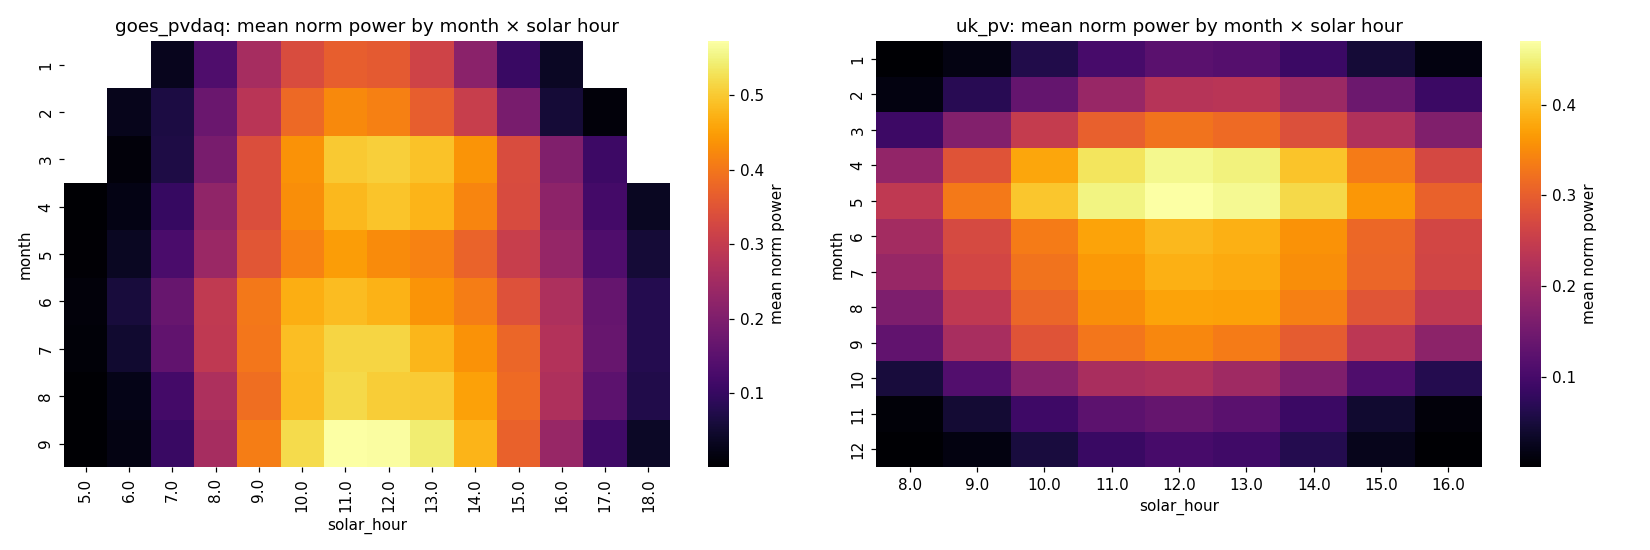
\includegraphics[width=0.90\textwidth]{figures/month_hour_heatmap.png}
\caption{How to read the heatmaps: rows are calendar months, columns are solar hours, and each cell gives mean normalized generation, with lighter colors denoting higher output. The panels show the regular daily profile and its seasonal change in each track.}
\label{fig:month-hour}
\end{figure}

Figure~\ref{fig:feature-power} shows the remaining uncertainty from another view. Each panel groups daytime observations by one numerical feature and normalized power, with color indicating the logarithmic number of observations in each hexagon. The denser regions reveal broad relationships between power and radiation, cloud cover, or temperature. The substantial vertical spread at many feature values shows that no one of these variables fixes the output. A forecaster must capture the regular solar envelope and respond to the local conditions that move power above or below it. An average daily error alone can obscure failures in this second task.

\begin{figure}[H]
\centering
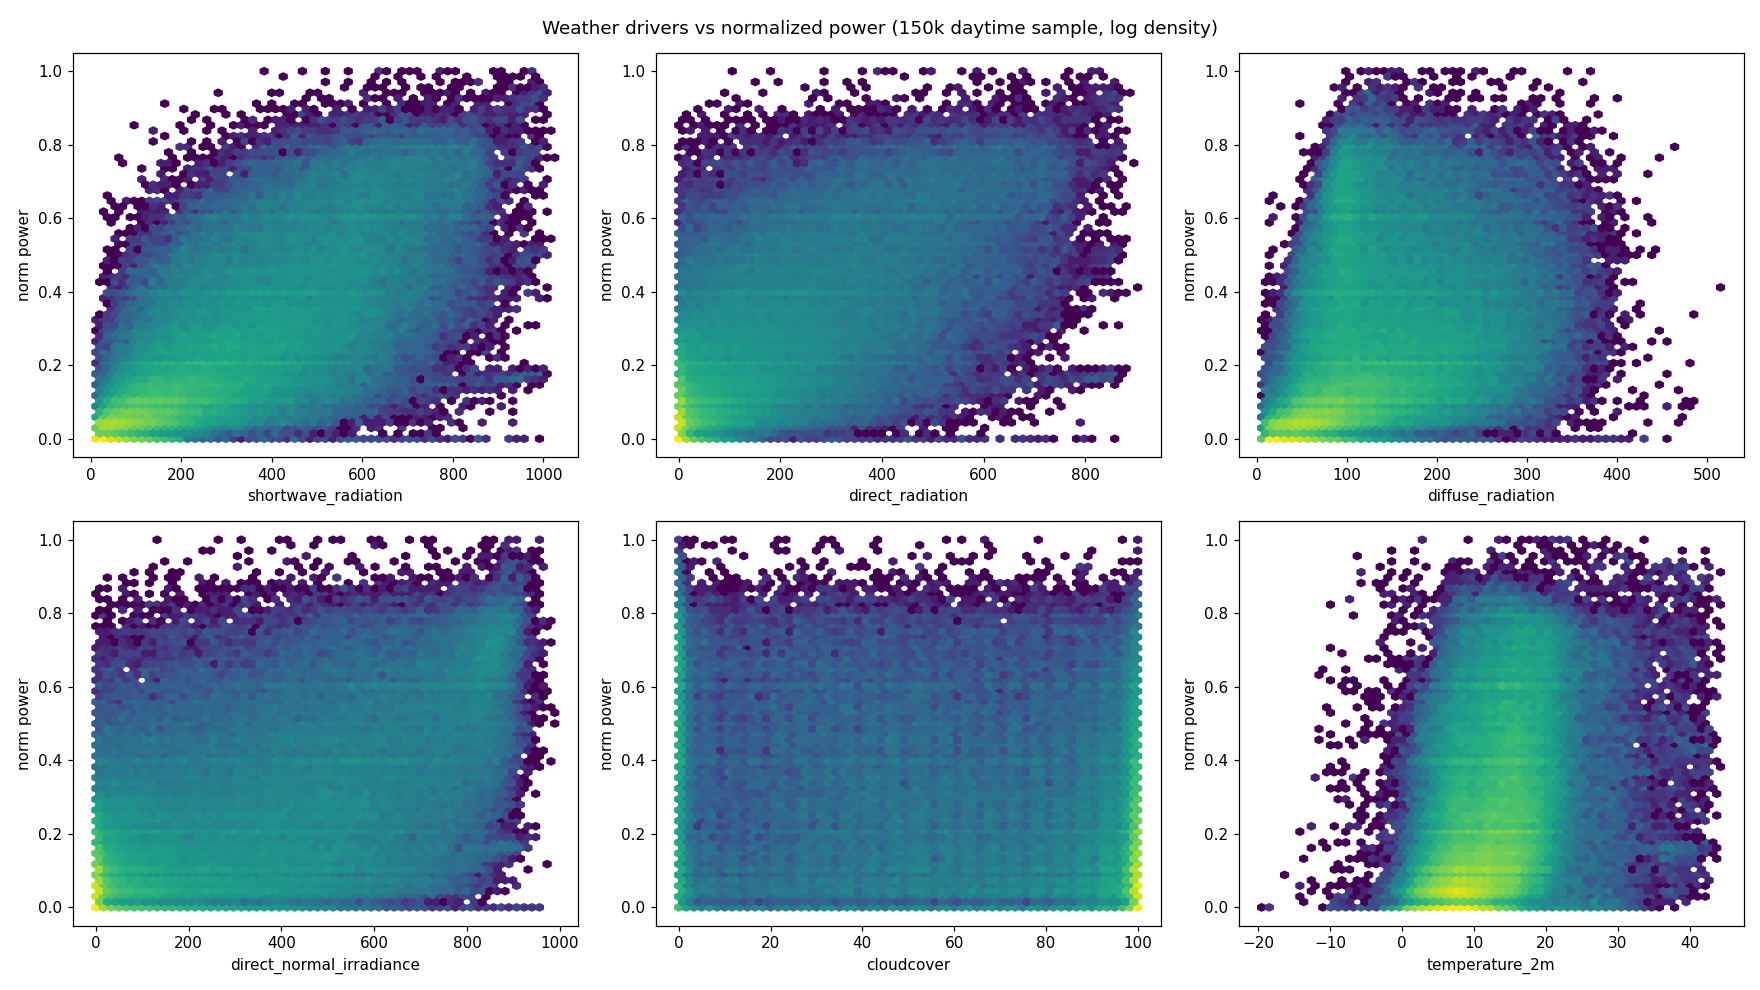
\includegraphics[width=0.90\textwidth]{figures/feature_vs_power_hexbin.png}
\caption{How to read the hexbin plots: each panel groups daytime observations by a numerical feature and normalized power. Color denotes the logarithmic number of observations in a bin. Broad vertical spread at a given feature value shows residual uncertainty beyond that individual feature.}
\label{fig:feature-power}
\end{figure}

\subsection{Ramps and the role of visual context}

Ramps are the signed changes in normalized power between successive valid daytime observations. Figure~\ref{fig:ramp-rates} has one panel for each track. The horizontal axis gives the change per native power step: negative values are drops in production, positive values are rises, and zero means that production changed little. The vertical axis counts observations on a logarithmic scale, showing the large mass of small changes and the relatively rare steep changes. Values outside the displayed interval are placed at $-0.5$ or $0.5$; the outermost bars therefore include all larger changes.

Both distributions peak sharply around zero, showing that most adjacent observations are similar. Their tails show the less frequent ramps that are harder to forecast and can dominate short-horizon errors. The figure describes the data, not a model result. Chapter~\ref{cha:protocol} defines how these observations become a scored ramp subset.

\begin{figure}[H]
\centering
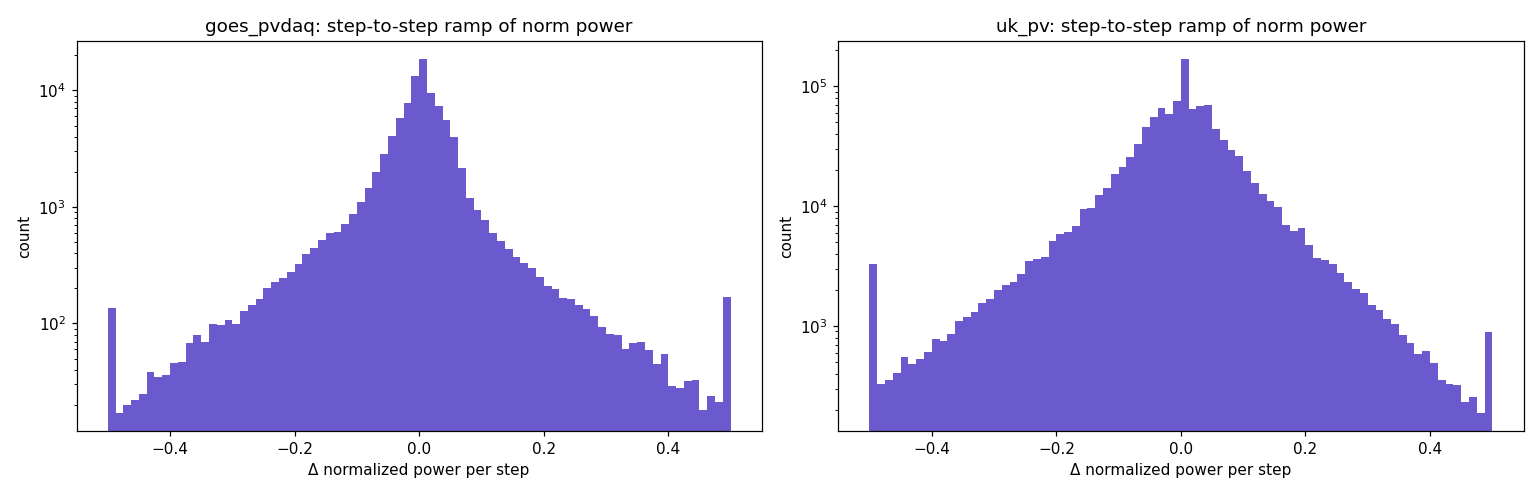
\includegraphics[width=0.90\textwidth]{figures/ramp_rates.png}
\caption{How to read the ramp distributions: the horizontal axis is the signed change in normalized power between successive daytime observations. The vertical axis is the logarithmic count of those changes. Values beyond $-0.5$ and $0.5$ are placed at the endpoints. The central peak contains stable intervals; the tails contain rapid changes.}
\label{fig:ramp-rates}
\end{figure}

A satellite frame does not make every ramp predictable. A cloud may form outside the crop, move in a direction the model cannot infer, or affect a panel differently from its surroundings. The figure nevertheless defines a narrow test: if recent visual structure adds information beyond numerical history, its benefit should be most apparent during these rapid transitions.

\subsection{Spatial and operational heterogeneity}

Capacity normalization places power on a common scale while preserving differences between plants. Figure~\ref{fig:site-context} shows these differences in two ways. In the capacity histograms, the horizontal axis is installed capacity and the vertical axis is the number of sites. UK systems occupy a narrow residential range, while the US track spans a much wider range. In the maps, each point is a plant; point size increases with the square root of capacity, and color gives mean normalized power. The sites are distributed across distinct geographic settings, and some UK plants lie close enough to share broad weather systems.

\begin{figure}[H]
\centering
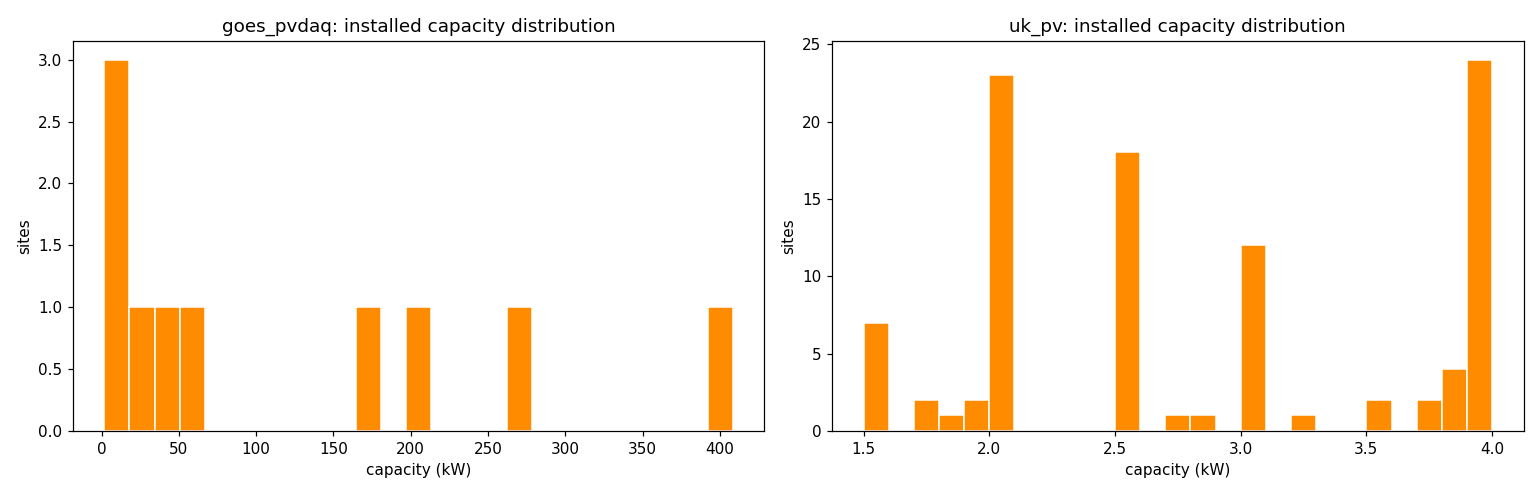
\includegraphics[width=0.49\textwidth]{figures/capacity_distribution.png}\hfill
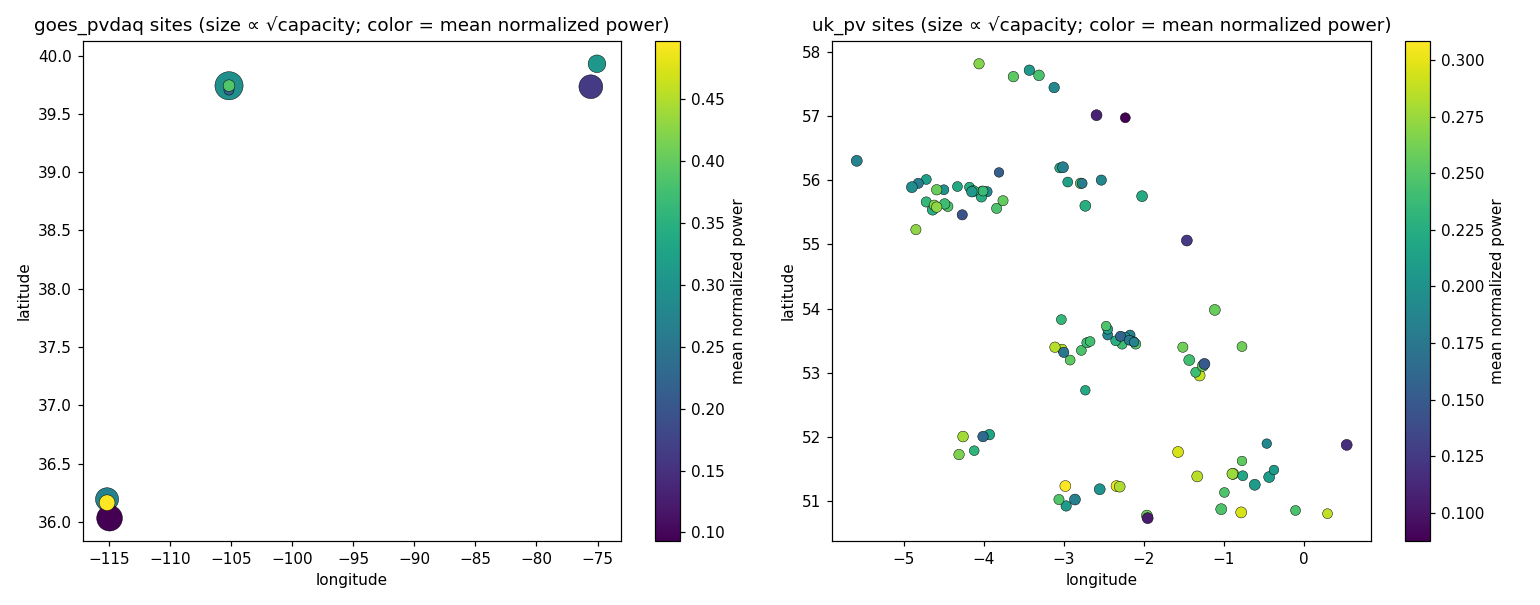
\includegraphics[width=0.49\textwidth]{figures/site_map.png}
\caption{Capacity distributions occupy the left block and plant maps the right block. Within each block, US sites appear on the left and UK sites on the right. Map-marker size is proportional to the square root of capacity; color denotes mean normalized power.}
\label{fig:site-context}
\end{figure}

Figure~\ref{fig:site-boxplot} compares the daytime normalized-power distributions of all 10 US plants and a fixed random sample of 15 UK plants. Plants are ordered by their median output. Within each box, the center line is the median and the box covers the middle half of observations. The different levels and spreads show that capacity normalization standardizes units without removing differences in local conditions and plant behavior.

\begin{figure}[H]
\centering
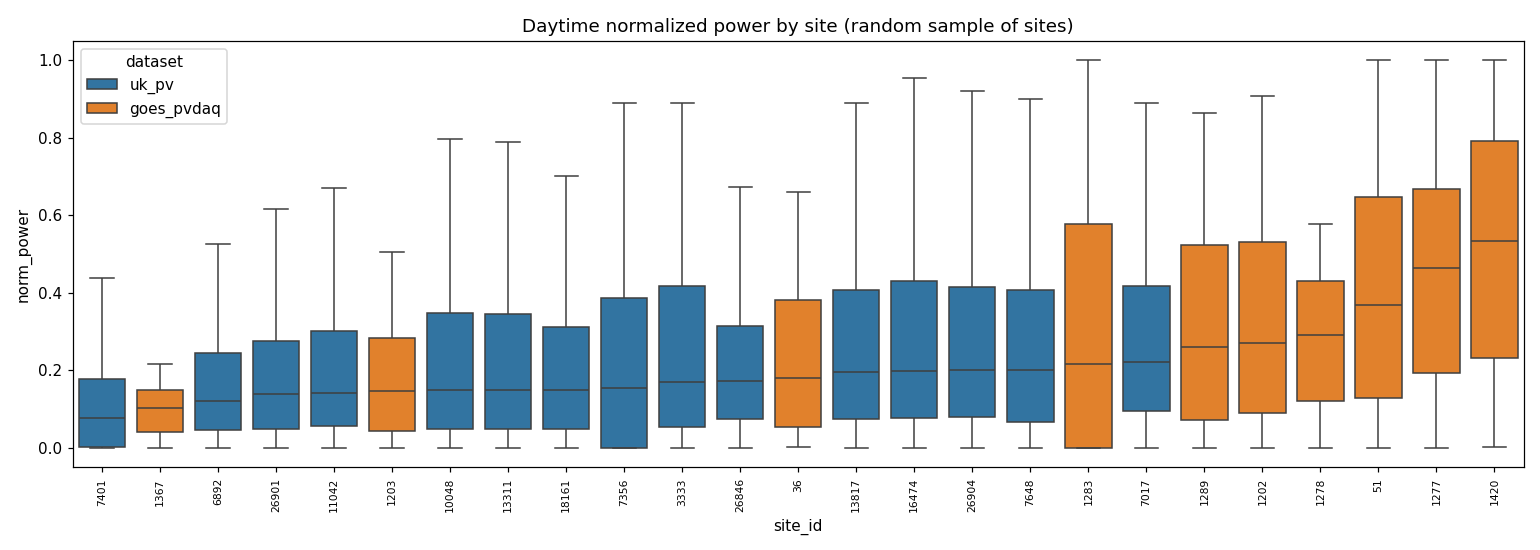
\includegraphics[width=0.94\textwidth]{figures/site_norm_power_boxplot.png}
\caption{Daytime normalized-power distributions by plant, showing all US sites and a fixed random sample of UK sites. Plants are ordered by median normalized power.}
\label{fig:site-boxplot}
\end{figure}

Figure~\ref{fig:covariate-correlations} summarizes the numerical inputs across all daytime observations. Rows and columns identify variables, and each cell gives the correlation for that pair; warmer colors indicate positive relationships and cooler colors negative ones. The left matrix uses Pearson correlation to measure linear association. The right uses rank-based Spearman correlation. Radiation variables are strongly positively associated with normalized power, whereas cloud cover is negatively associated. These pooled relationships provide useful context. Site-specific variation motivates plant-disjoint evaluation, while the next analysis examines temporal persistence within individual series.

\begin{figure}[H]
\centering
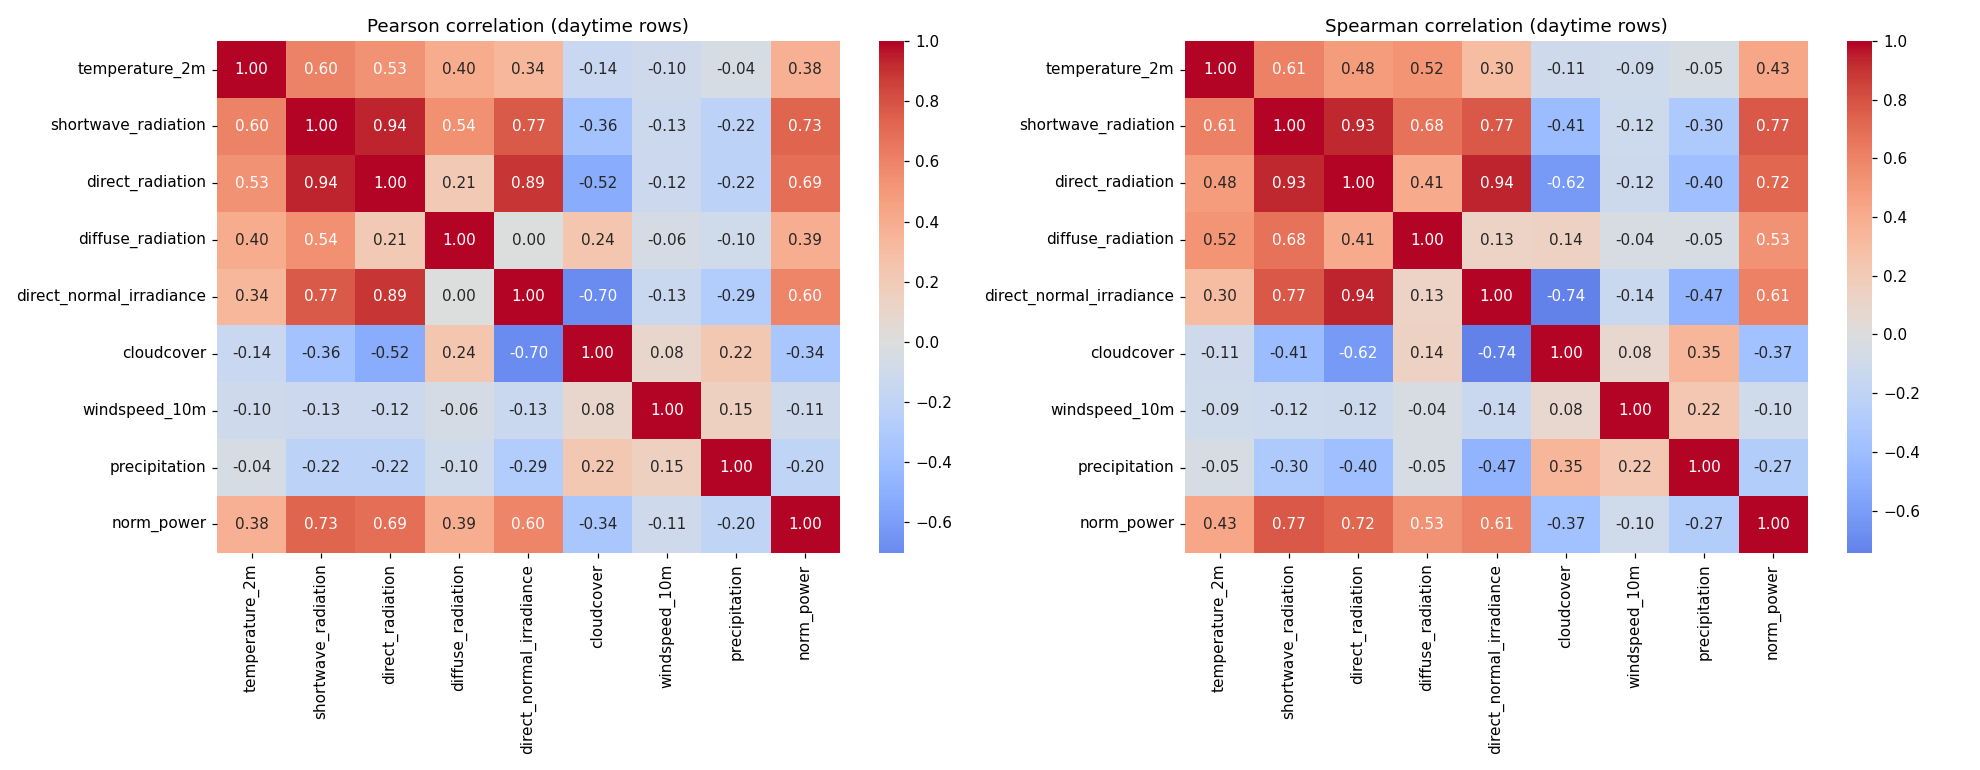
\includegraphics[width=0.92\textwidth]{figures/correlation_matrices.png}
\caption{Pearson (left) and Spearman (right) correlations among numerical covariates and normalized power over daytime observations.}
\label{fig:covariate-correlations}
\end{figure}

\subsection{Persistence and the choice of context length}

Figure~\ref{fig:power-acf} has two views of autocorrelation for PVDAQ plant 1420 and UKPV plant 6966. The left panel covers the first six hours, with lag on the horizontal axis and autocorrelation on the vertical axis. Both lines begin close to one, so persistence is a demanding reference forecast at short horizons. The US correlation reaches zero at about three hours and then becomes negative as the comparison crosses to the opposite side of the daily cycle. The UK correlation declines more gradually. It reaches about one half after three hours and remains near one third at six hours.

The right panel extends the same calculation over the full fourteen-day history. Both tracks show repeating daily peaks. At a one-day lag, autocorrelation is 0.822 for PVDAQ and 0.609 for UKPV. At fourteen days, it is 0.783 and 0.530, respectively. The recurring pattern supports the use of several daily profiles in the context window. The intraday decline shows why recent power alone is insufficient for the later forecast horizon.

\begin{figure}[H]
\centering
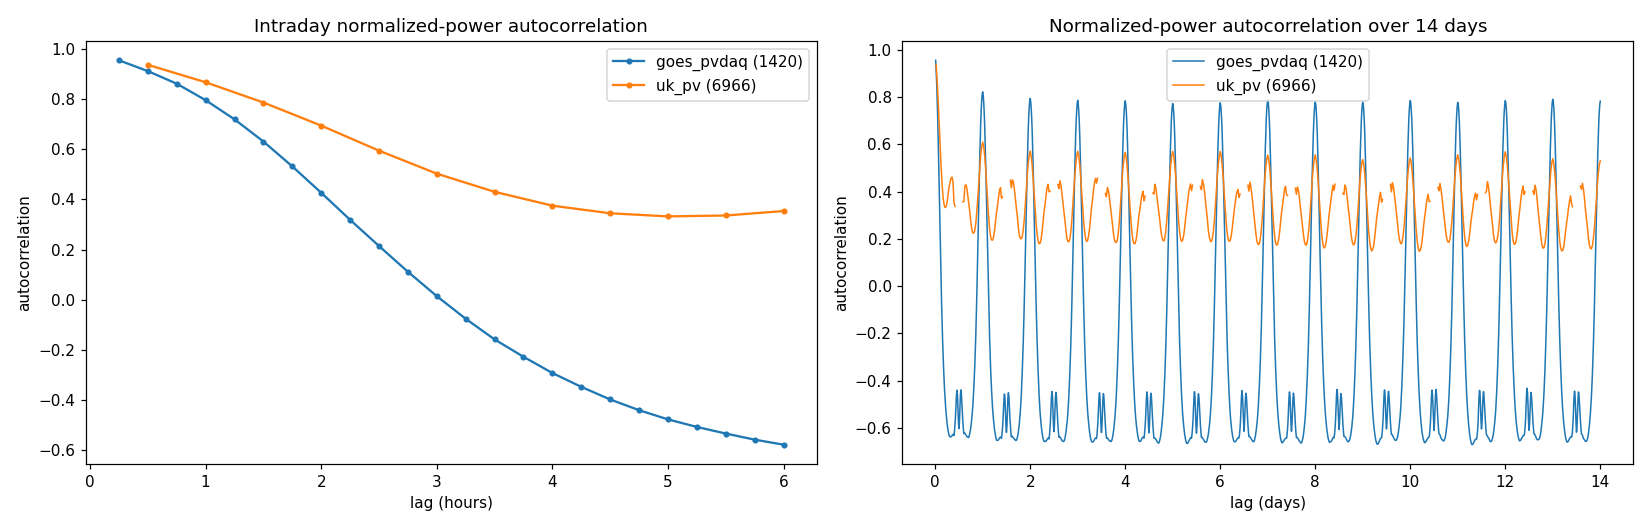
\includegraphics[width=0.92\textwidth]{figures/power_acf.png}
\caption{Normalized-power autocorrelation at PVDAQ plant 1420 and UKPV plant 6966, shown over the first six hours (left) and the full fourteen-day context window (right).}
\label{fig:power-acf}
\end{figure}

The model therefore receives fourteen days of history. This window gives it repeated observations of the same plant at the same clock time under different weather conditions. It still provides context when the most recent intervals are missing. For the UK track, fourteen days contain 672 half-hour observations. Chronos-2 reduces them to 42 temporal tokens before fusion. A longer window would add more tokens and missing intervals; a shorter one would make the forecast depend more heavily on a single recent daily profile. The ablations measure whether this context improves forecasting.

\subsection{Unequal contribution across plants}

Plants contribute unequal amounts of data because their records do not cover the same number of calendar days. Site coverage is measured from a plant's first to its last timestamp: it is the fraction of days in that span for which the corpus retains at least one observation. This measure is appropriate for the daytime-only record, where nights are absent by design. Figure~\ref{fig:site-coverage} groups plants by that percentage, with each bar giving the number of plants in a coverage range. UK coverage is tightly concentrated between 99.3\% and 100\%, whereas PVDAQ coverage ranges from 71.8\% to 100\%.

\begin{figure}[H]
\centering
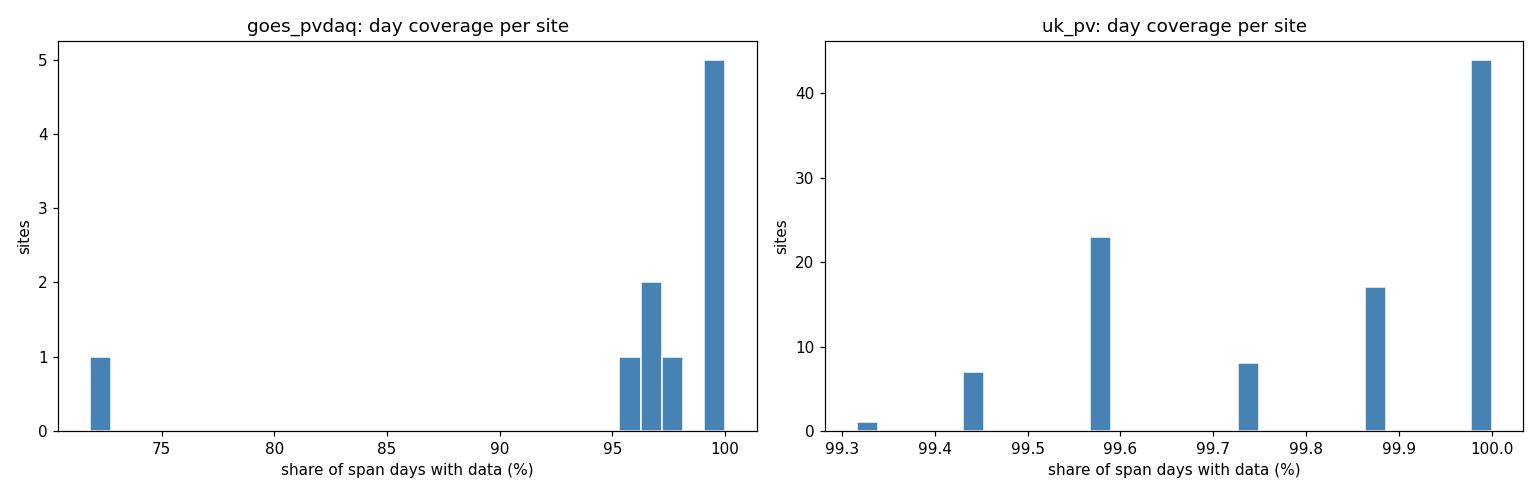
\includegraphics[width=0.92\textwidth]{figures/coverage_per_site.png}
\caption{Share of active-span days containing observations for each plant in the US and UK tracks.}
\label{fig:site-coverage}
\end{figure}

Figure~\ref{fig:site-behavior} summarizes two aspects of daytime behavior by plant. The left histogram gives mean normalized power, and the right gives its Pearson correlation with shortwave radiation. The distributions show that plants differ in typical output and in their numerical relationship with radiation. This variation motivates the plant-level aggregation rule in Chapter~\ref{cha:protocol}.

\begin{figure}[H]
\centering
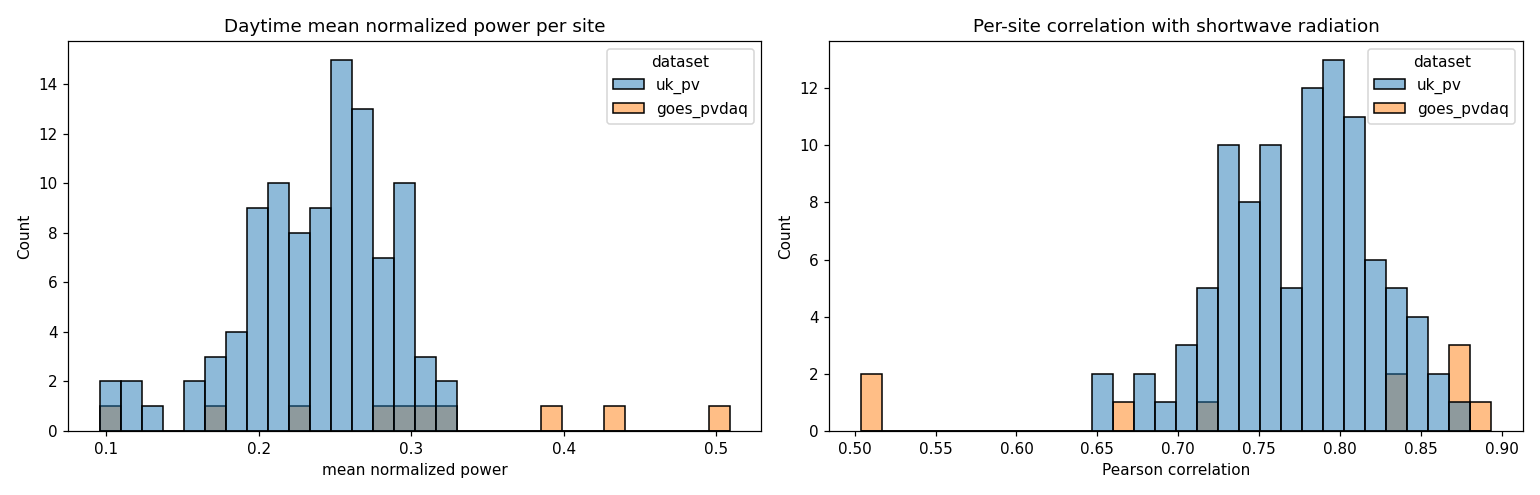
\includegraphics[width=0.92\textwidth]{figures/site_capacity_factor_and_corr.png}
\caption{Per-plant distributions of daytime mean normalized power (left) and Pearson correlation between normalized power and shortwave radiation (right).}
\label{fig:site-behavior}
\end{figure}

\subsection{Seasonal and target imbalance}

The two tracks cover different seasonal ranges. UKPV includes all of 2019 and 2020, whereas PVDAQ ends in September 2019. The target distribution therefore combines the daily production cycle with the months represented in each source.

Figure~\ref{fig:target-distribution} shows this distribution in three forms. The first histogram includes all retained rows and has a large concentration near zero. The second restricts the sample to producing rows, revealing the distribution once near-zero values are excluded. The third shows absolute power on a logarithmic scale. This view makes the wide difference in physical scale across plants visible. High normalized output occurs less often than low output.

\begin{figure}[H]
\centering
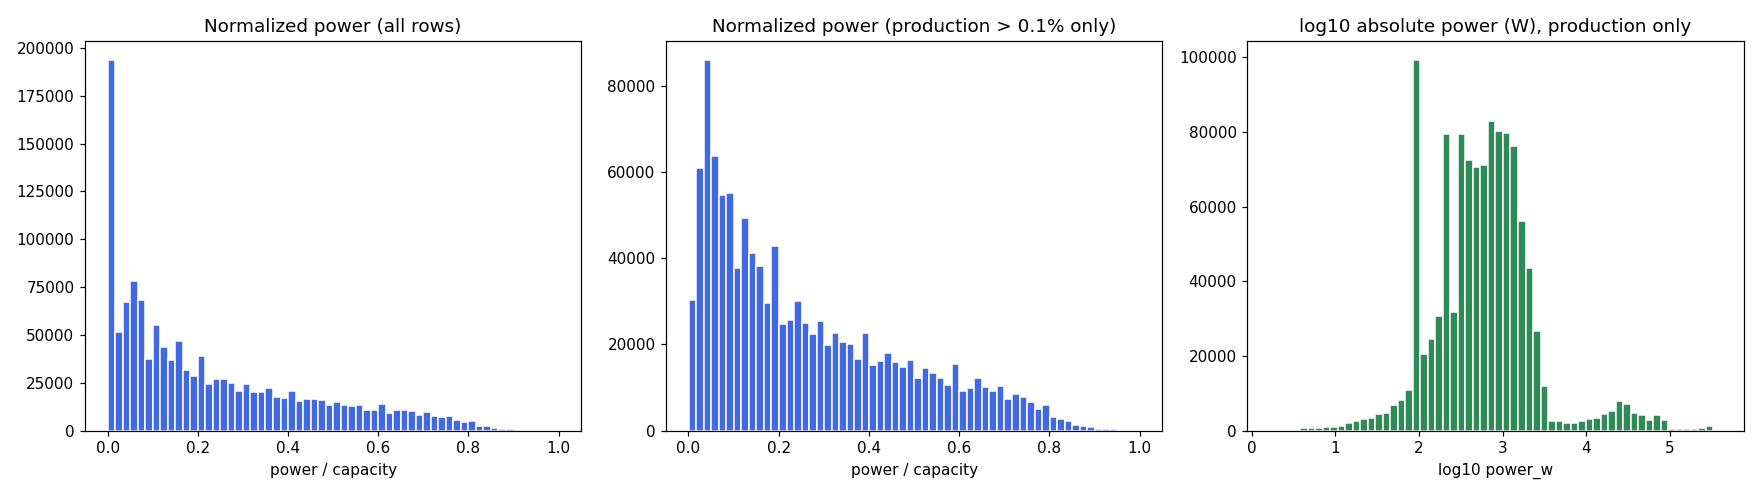
\includegraphics[width=0.92\textwidth]{figures/power_distributions.png}
\caption{Normalized-power distributions over all retained rows (left) and producing rows (center), with the distribution of absolute power on a logarithmic scale (right).}
\label{fig:target-distribution}
\end{figure}

Figure~\ref{fig:monthly-production} plots mean normalized power for each calendar month. The UK line traces two full annual cycles, while the PVDAQ line covers January through September 2019. Production rises through spring, is higher during summer months, and falls again toward winter. The two lines should be read in light of their different geographic settings and time coverage. The next analysis narrows from these seasonal patterns to whether cloud cover explains variation within irradiance ranges.

\begin{figure}[H]
\centering
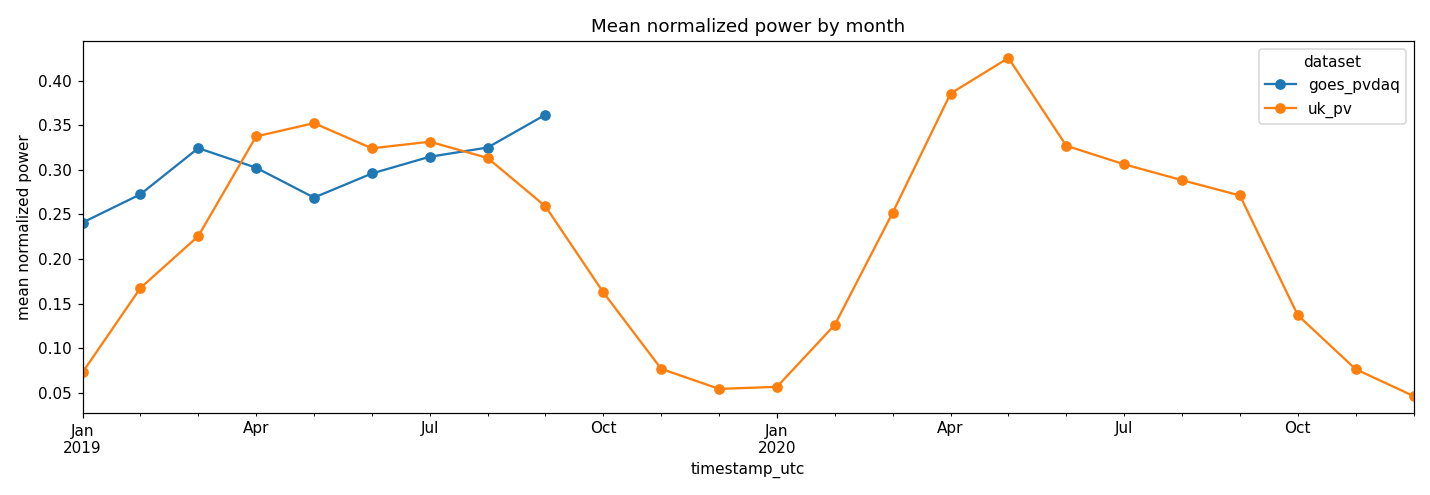
\includegraphics[width=0.92\textwidth]{figures/monthly_production.png}
\caption{Mean normalized power by calendar month for UKPV and PVDAQ.}
\label{fig:monthly-production}
\end{figure}

\subsection{What numerical cloud cover leaves unexplained}

The numerical record already includes cloud-related covariates. The relevant question is whether uncertainty remains after those covariates are known. Figure~\ref{fig:cloud-residual} conditions on shortwave radiation by grouping observations into five irradiance ranges. Within each range, it separates reanalysis cloud cover into clear, mixed, and overcast categories. Each box summarizes normalized power in one group: the center line is the median and the box spans the middle half of observations.

Within the displayed irradiance ranges, clearer categories generally have higher median output than overcast categories. This descriptive association motivates testing cloud-related inputs alongside irradiance. The broad bins and pooled plants leave any independent predictive contribution unmeasured. The boxes also overlap broadly, showing that these scalar covariates leave realized output variable.

\begin{figure}[H]
\centering
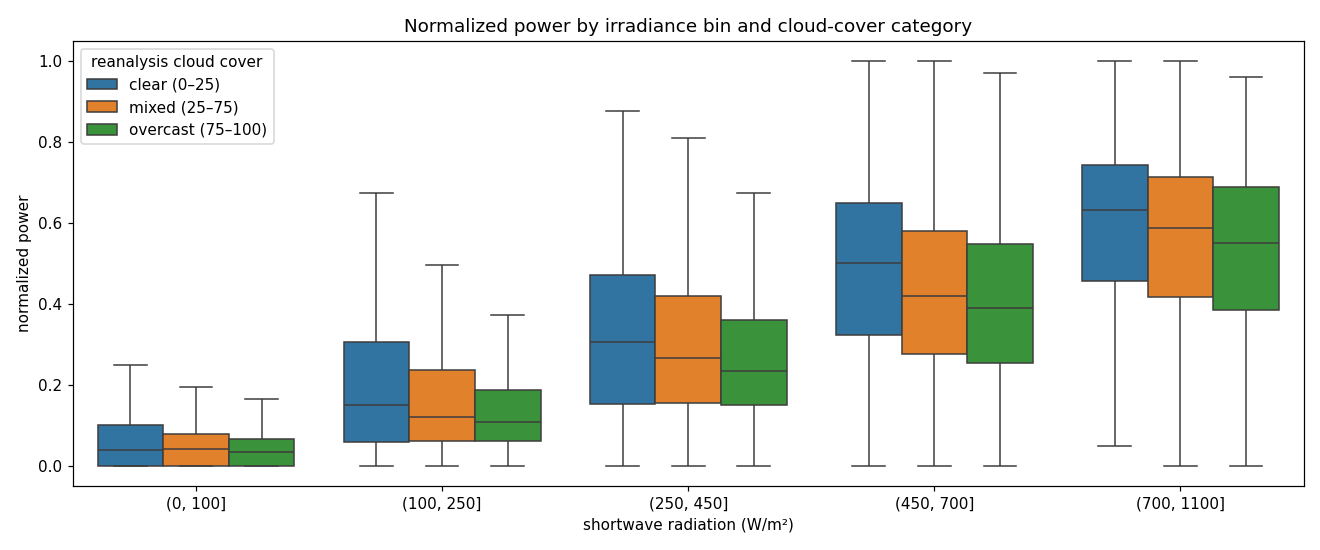
\includegraphics[width=0.92\textwidth]{figures/cloudcover_residual_effect.png}
\caption{Daytime normalized power within shortwave-radiation ranges, separated by reanalysis cloud-cover category.}
\label{fig:cloud-residual}
\end{figure}

The boxes summarize observed groups after conditioning on irradiance and cloud cover. Their residual spread may reflect plant behavior, measurement error, or weather outside the image crop. The method and evaluation chapters test whether an independent visual input explains part of that variation.
